\chapter[Algorithms]{Algorithms}
\label{chap:algorithms}

Building on the foundational understanding of gravitational lensing and its computational challenges, a critical aspect of modern astrophysical research involves the optimization of parametric functions to model the complex phenomena of the Universe accurately. This optimization is essential in gravitational lensing studies, where precise models of the mass distribution within lensing objects are paramount for interpreting the observed lensing effects. The optimization process often requires navigating a high-dimensional parameter space to find the best-fit parameters that reconcile theoretical models with observational data, a task that can be computationally intensive and algorithmically complex.

In this context, the advent of frameworks such as PyTorch\footnote{\url{https://pytorch.org}} \citep{paszke_pytorch_2019} and TensorFlow\footnote{\url{https://www.tensorflow.org}} \citep{abadi_tensorflow_2016} represents a significant leap forward for astrophysical research. These open-source libraries, primarily developed for deep learning applications, offer powerful tools for automatic differentiation, a technique that facilitates the calculation of gradients automatically, a cornerstone for any optimization algorithm. The ability of PyTorch and TensorFlow to efficiently compute derivatives of highly complex, nested functions makes them exceptionally well suited for optimizing parametric models in gravitational lensing studies.

Moreover, PyTorch and TensorFlow are designed to exploit the capabilities of modern computing hardware, including GPUs and TPUs, enabling the parallel processing of large datasets and the acceleration of computational tasks. This feature is particularly beneficial for gravitational lensing research, where handling large amounts of observational data and running complex simulations is commonplace. Using the computational power offered by these frameworks, one can significantly reduce the time required for model optimization and data analysis, thus enhancing the efficiency of the investigations.

% *************************************************************
%%%%% SECTION 4.1: DIFFERENTIABLE PROGRAMMING %%%%%
%%%%%%%%%%%%%%%%%%%%%%%%%%%%%%%%%%%%%%%%%%%%%%%%%%%%%%%
%%%%% Sec: Differentiable programming %%%%%
%%%%%%%%%%%%%%%%%%%%%%%%%%%%%%%%%%%%%%%%%%%%%%%%%%%%%%%
\section{Differentiable programming}
\label{sec:diff_prog}

Differentiable programming is an advanced computational paradigm that unites traditional programming concepts with the principles of differentiation, a fundamental concept in calculus. This approach extends the idea of computing derivatives to entire programs, enabling the automatic calculation of gradients of program outputs with respect to inputs. Differentiable programming is particularly powerful in the context of optimization, machine learning, and artificial intelligence, where it facilitates efficient parameter tuning to minimize or maximize some objective function.
Methods for computing derivatives in computer programs can be classified into four categories (see \cref{fig:diff_methods}):
\begin{enumerate}
    \item manually working out derivatives and coding them;
    \item \textbf{numerical differentiation}, involves approximating the derivative of a function using values of the original function evaluated at some sample points \citep{burden_numerical_2016}. In its simplest form, it is based on the limit definition of a derivative. It is quite simple to implement and apply to a wide range of problems, especially when dealing with data-driven models or functions that lack a clear analytical representation. Its effectiveness diminishes in high-dimensional settings, where the complexity and computational demands increase exponentially, highlighting the method's limitations in handling complex, multi-variable functions efficiently;
    \item \textbf{symbolic differentiation}, which refers to the automatic process of finding derivatives using the rules of differentiation to obtain an exact symbolic expression for the derivative of a given function \citep{grabmeier_computer_2003}. This method works similarly to how humans perform differentiation ``by hand'', manipulating symbols according to mathematical laws;
    \item \textbf{automatic differentiation} (AD), also called algorithmic differentiation,is a method that computes the derivative of a function efficiently and accurately by systematically applying the chain rule of calculus to the sequence of elementary operations (additions, multiplications, trigonometric functions, etc.) that constitute a computer program. All numerical computations are ultimately compositions of a finite set of elementary operations for which derivatives are known \citep{verma_introduction_2000,griewank_evaluating_2008}, and combining the derivatives of the constituent operations through the chain rule of calculus\footnote{The derivative of the composition of two (or more) differentiable functions $f$ and $g$ can be expressed in terms of the derivatives of the single functions $f$ and $g$. If $h (x) = f(g(x))$, then $h^\prime(x) = f^\prime(g(x)) g^\prime(x)$.} gives the derivative of the overall composition. AD is not an approximation like numerical differentiation, but rather computes derivatives to machine precision.
\end{enumerate}
\newpage
In particular, differentiable programming refers to using automatic differentiation in some way that allows a program to optimize its parameters to improve on some task. It only has three requirements:
\begin{enumerate}
    \item a parameterized function/model to be optimized;
    \item (automatic) differentiability of the object to be optimized;
    \item a function suitable to measure the performance of the model.
\end{enumerate}

The process of optimizing a model in the field of differentiable programming is often called \emph{training}.
In the subsequent portion of this section, a comprehensive overview of automatic differentiation and its role in the training process will be provided. This will be followed by an in-depth exposition of the process itself.

\begin{figure}
    \centering
    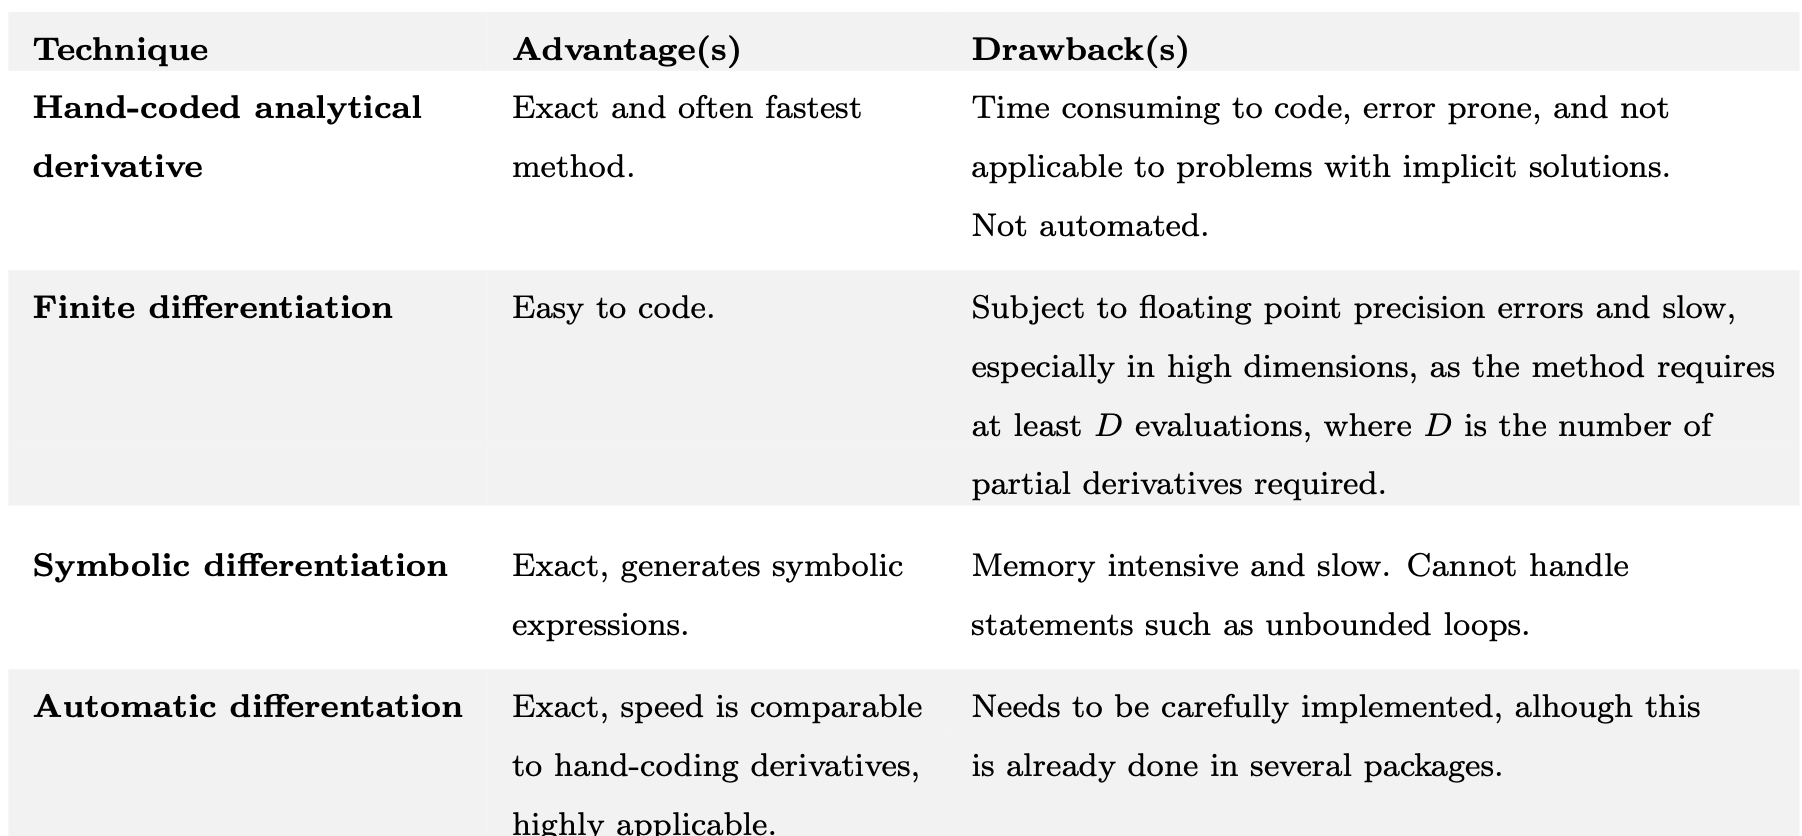
\includegraphics[width=\linewidth, keepaspectratio]{img//chapter4/diff_methods.png}
    \caption[Summary of techniques to calculate derivatives]{Summary of techniques to calculate derivatives.\\\small{Credits: \cite{margossian_review_2019}.}}
    \label{fig:diff_methods}
\end{figure}


%%%%%%%%%%%%%%%%%%%%%%%%%%%%%%%%%%%%%%%%%%%%%%%%%%%%%%%
%%%%% SubSec: Automatic differentiation %%%%%
%%%%%%%%%%%%%%%%%%%%%%%%%%%%%%%%%%%%%%%%%%%%%%%%%%%%%%%
\subsection{Automatic differentiation}
\label{subsec:automatic_differentiation}


%%%%%%%%%%%%%%%%%%%%%%%%%%%%%%%%%%%%%%%%%%%%%%%%%%%%%%%
%%%%% SubSubSec: Computational graph %%%%%
%%%%%%%%%%%%%%%%%%%%%%%%%%%%%%%%%%%%%%%%%%%%%%%%%%%%%%%
\subsubsection{Computational graph}
\label{subsubsec:computational_graph}
As already stated, automatic differentiation operates on the fundamental principle that complex functions can be decomposed into a series of elementary arithmetic operations. Given a target composite function $f (x) = h \circ g(x) = h(g(x))$, with $x \in \mathbb{R}^n$, $g : \mathbb{R}^n \rightarrow \mathbb{R}^k$, and $h : \mathbb{R}^k \rightarrow \mathbb{R}^m$, applying the chain rule and elementary matrix multiplication, the corresponding Jacobian matrix\footnote{The Jacobian matrix of a vector-valued function of several variables is the matrix of all its first-order partial derivatives.} $J$ is thus:
\be
\label{eq:4.1}
J = J_{h \circ g} = J_h (g(x)) \cdot J_g (x) \,,
\ee
with $(i,j)^{th}$ element:
\be
\label{eq:4.2}
J_{ij} = \frac{\partial f_i}{\partial x_j} = \frac{\partial h_i}{\partial g_1} \frac{\partial g_1}{\partial x_j} + \frac{\partial h_i}{\partial g_2} \frac{\partial g_2}{\partial x_j} + \ldots + \frac{\partial h_i}{\partial g_k} \frac{\partial g_k}{\partial x_j} \,.
\ee

More generally, if $f$ is the composite expression of $L$ functions
\be
\label{eq:4.3}
f = f^L \circ f^{L-1} \circ \ldots \circ f^1 \,,
\ee
the corresponding Jacobian matrix will be
\be
\label{eq:4.4}
J = J_L \cdot J_{L-1} \cdot \ldots \cdot J_1 \,.
\ee
Hence, given a complex function $f$, it is possible to break down the action of the Jacobian matrix on a vector into simple components.
So, following \cite{griewank_evaluating_2008} notation, a function $f : \mathbb{R}^n \rightarrow \mathbb{R}^m$ can be constructed using intermediate variables $v_i$ such that
\begin{itemize}
    \item variables $v_{i-n} = x_i$, $i = 1, \ldots, n$ are the input variables,
    \item variables $v_{i}$, $i = 1, \ldots, l$ are the intermediate variables,
    \item variables $y_{m-i} = v_{l-i}$, $i = m-1, \ldots, 0$ are the output variables.
\end{itemize}
The representation of all the elementary operations that take place to construct a certain function $f$ is called the \emph{evaluation trace}, which can also be pictured as a \emph{computational graph} \citep{bauer_computational_1974}, useful for visualizing the dependency relations between intermediate variables. \Cref{fig:computational_graph} shows the computation graph for an example function $f : \mathbb{R}^2 \rightarrow \mathbb{R}$: 
\be
\label{eq:4.5}
f(x_1, x_2) = \ln{(x_1)} + x_1 x_2 - \sin{(x_2)} \,.
\ee

\begin{figure}
    \centering
    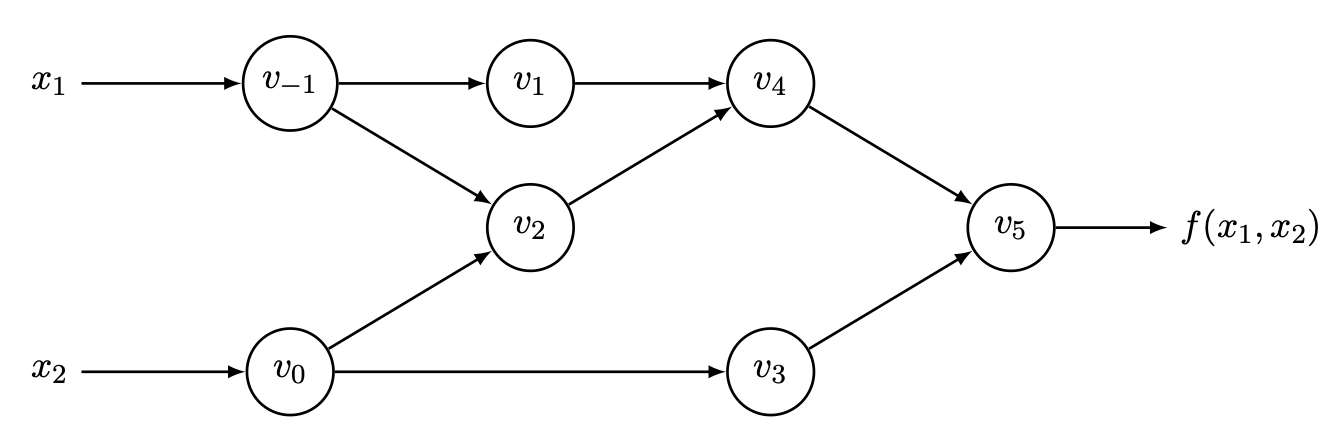
\includegraphics[width=0.9\linewidth, keepaspectratio]{img//chapter4/computational_graph.png}
    \caption[Example of computational graph]{Computational graph of the example $f(x_1, x_2) = \ln{(x_1)} + x_1 x_2 - \sin{(x_2)}$.\\\small{Credits: \cite{baydin_automatic_2018}.}}
    \label{fig:computational_graph}
\end{figure}

Given the computational graph of all elementary operations, AD can be implemented in two main modes: \emph{forward} accumulation mode and \emph{reverse} accumulation mode (backward mode).


%%%%%%%%%%%%%%%%%%%%%%%%%%%%%%%%%%%%%%%%%%%%%%%%%%%%%%%
%%%%% SubSubSec: Forward mode %%%%%
%%%%%%%%%%%%%%%%%%%%%%%%%%%%%%%%%%%%%%%%%%%%%%%%%%%%%%%
\subsubsection{Forward mode}
\label{subsubsec:forward_mode}
Automatic differentiation in forward accumulation mode (or \emph{tangent linear} mode) is the conceptually most simple type. The differentiation process is aligned with the function evaluation itself. Starting from the inputs, the program computes both the function's value and its derivative step by step through the computation graph. For each elementary operation, the forward mode calculates the derivative of the output with respect to the inputs, carrying these derivatives (or ``tangents'') forward through the computation graph.

Considering as an example the evaluation trace of the function defined in \cref{eq:4.5} (left-hand side of \cref{fig:forward_trace}), for computing the derivative of $f$ with respect to $x_1$, the first step is to associate with each intermediate variable $v_i$ a derivative
\be
\label{eq:4.6}
\Dot{v}_i = \frac{\partial v_i}{\partial x_1}.
\ee

Applying then the chain rule to each elementary operation in the forward primal trace, the corresponding tangent (derivative) trace is generated (right-hand side of \cref{fig:forward_trace}), until the required derivative in the final variable $\Dot{v}_5 = \frac{\partial y}{\partial x_1}$ is obtained.

Generalizing this procedure to a function $f : \mathbb{R}^n \rightarrow \mathbb{R}^m$, each forward pass of AD provides one column of the Jacobian matrix (\ie the partial derivatives of all output variables with respect to one input variable).
Thus, the complete Jacobian can be computed in $n$ evaluations. For this reason, forward AD is efficient and straightforward especially for functions $f : \mathbb{R} \rightarrow \mathbb{R}^m$, for which all derivatives can be computed with just one forward pass.

In general, for functions with many inputs $f : \mathbb{R}^n \rightarrow \mathbb{R}^m$ where $n \gg m$, the reverse accumulation mode of AD is preferred.

\begin{figure}
    \centering
    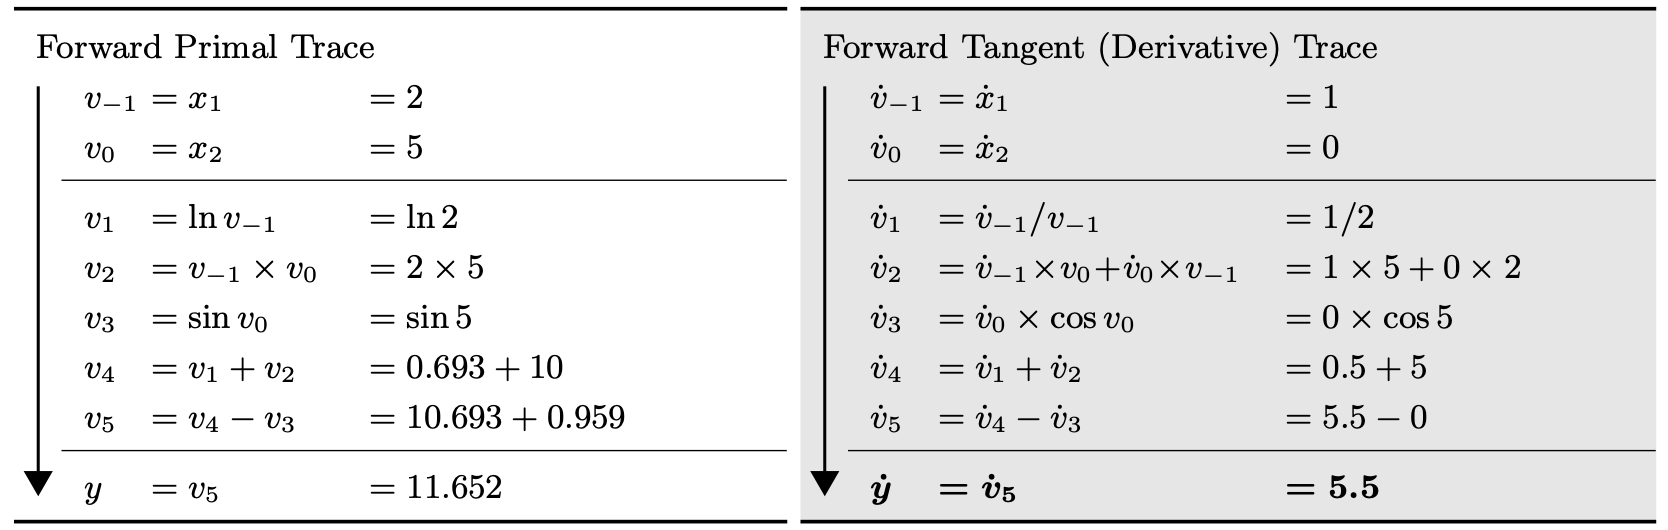
\includegraphics[width=\linewidth]{img//chapter4/forward_trace.png}
    \caption[Forward mode AD example]{Forward mode AD example for $f(x_1, x_2) = \ln{(x_1)} + x_1 x_2 - \sin{(x_2)}$, evaluated at $(x_1, x_2) = (2, 5)$ by setting $\Dot{x}_1 = 1$. The original forward evaluation of the primals on the left is augmented by the tangent operations on the right, where each line complements the original directly to its left.\\\small{Credits: \cite{baydin_automatic_2018}.}}
    \label{fig:forward_trace}
\end{figure}


%%%%%%%%%%%%%%%%%%%%%%%%%%%%%%%%%%%%%%%%%%%%%%%%%%%%%%%
%%%%% SubSubSec: Reverse mode %%%%%
%%%%%%%%%%%%%%%%%%%%%%%%%%%%%%%%%%%%%%%%%%%%%%%%%%%%%%%
\subsubsection{Reverse mode}
\label{subsubsec:reverse_mode}
AD in reverse accumulation mode (or \emph{adjoint} or \emph{cotangent linear} mode) \citep{griewank_numerical_2012} corresponds to a generalized backpropagation algorithm, in that it propagates derivatives backward from a given output. This is done by complementing each variable $v_i$ with an adjoint
\be
\label{eq:4.7}
\overline{v}_i = \frac{\partial y_j}{\partial v_i} \,,
\ee
which represents the sensitivity of a considered output $y_j$ with respect to changes in $v_i$.

In reverse mode AD, derivatives are computed in the second of a two-phase process. In the first phase, the original function code is run forward, creating intermediate variables $v_i$ and recording the dependencies in the computational graph. In the second phase, derivatives are calculated by propagating adjoints $\overline{v}_i$ in reverse, from outputs to inputs. The reverse mode AD for the example function of \cref{eq:4.5} is shown in \cref{fig:reverse_trace}.

An important advantage of the reverse mode is that it is significantly less costly to evaluate (in terms of operation count) than the forward mode for functions with a large number of inputs. In the extreme case of $f : \mathbb{R}^n \rightarrow \mathbb{R}$, only one application of the reverse
mode is sufficient to compute the full gradient, compared with the $n$ passes of the forward mode needed to populate the same. Because the optimization of astrophysical and gravitational lensing parametric functions usually involves the gradient of a scalar-valued objective with respect to a (large) number of parameters, this establishes the reverse mode, as opposed to the forward mode, as the mainstay technique in the form of the backpropagation algorithm \citep{schmidhuber_deep_2015}.

\begin{figure}
    \centering
    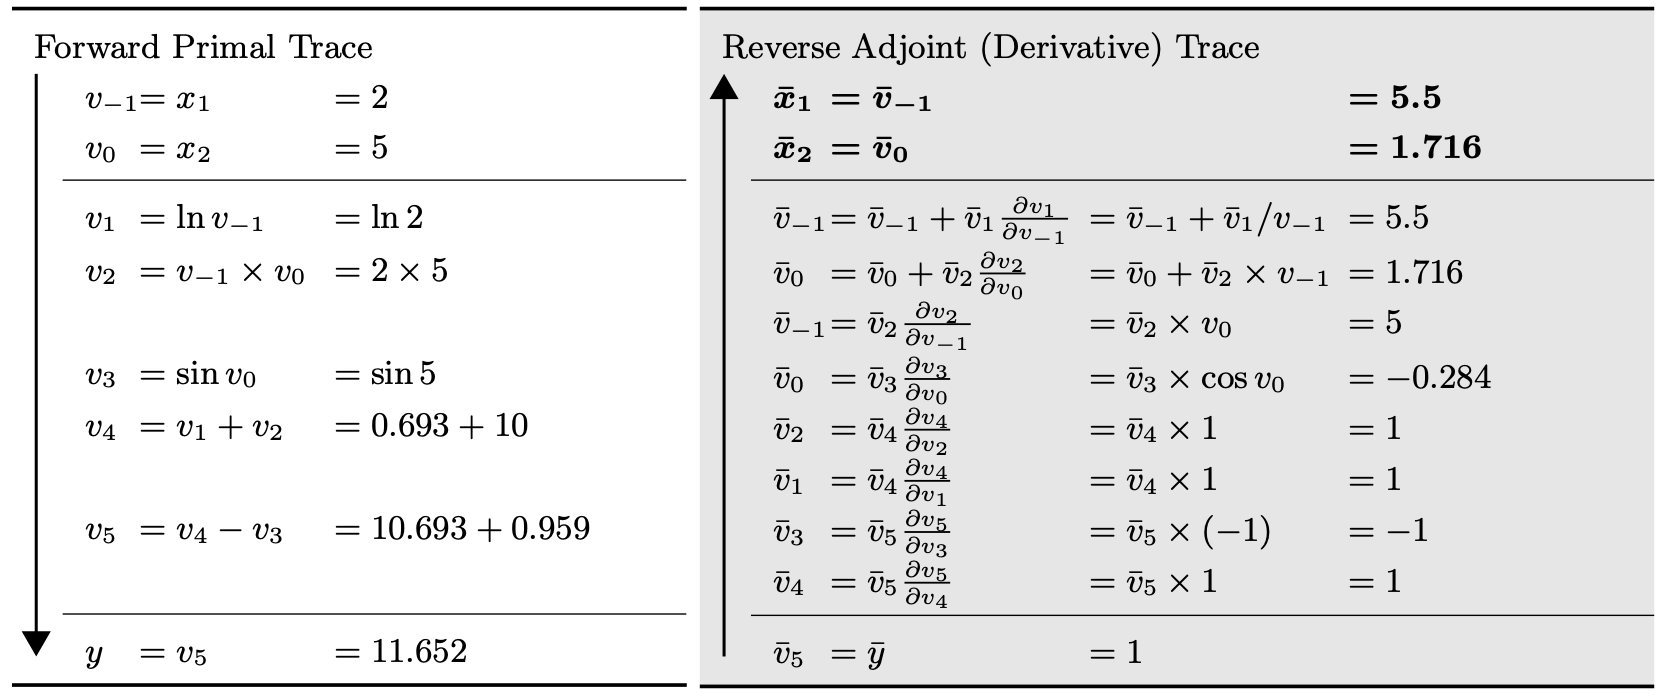
\includegraphics[width=0.9\linewidth, keepaspectratio]{img//chapter4/reverse_trace.png}
    \caption[Reverse mode AD example]{Reverse mode AD example for $f(x_1, x_2) = \ln{(x_1)} + x_1 x_2 - \sin{(x_2)}$, evaluated at $(x_1, x_2) = (2, 5)$. After forward evaluation of the primals on the left, adjoint operations on the right are evaluated in reverse.\\\small{Credits: \cite{baydin_automatic_2018}.}}
    \label{fig:reverse_trace}
\end{figure}


%%%%%%%%%%%%%%%%%%%%%%%%%%%%%%%%%%%%%%%%%%%%%%%%%%%%%%%
%%%%% SubSec: Backpropagation algorithm %%%%%
%%%%%%%%%%%%%%%%%%%%%%%%%%%%%%%%%%%%%%%%%%%%%%%%%%%%%%%
\subsection{Backpropagation algorithm}
\label{subsec:backpropagation_algorithm}
The backpropagation algorithm is the cornerstone of neural network training \citep{rumelhart_learning_1986,montavon_efficient_2012}, mainly used to minimize the error by adjusting the weights of the connections in the network. However, when it comes to a model optimization problem outside the realm of neural networks, such as training parametric models, the concept of backpropagation refers to the method of computing gradients efficiently using reverse mode AD.

The training process (or better, the training loop) is characterized by a sequence of operations performed recursively. The optimization itself is performed by an \emph{optimizer} which operates by tweaking the model parameters in a certain way, with the purpose of minimizing a \emph{loss} function, which quantifies the difference between the predicted outputs of the model and the actual target/observed values. 
The main algorithm that allows for this optimization is the so-called \emph{gradient descent.}


%%%%%%%%%%%%%%%%%%%%%%%%%%%%%%%%%%%%%%%%%%%%%%%%%%%%%%%
%%%%% SubSubSec: Loss function %%%%%
%%%%%%%%%%%%%%%%%%%%%%%%%%%%%%%%%%%%%%%%%%%%%%%%%%%%%%%
\subsubsection{Loss function}
\label{subsubsec:loss_func}
As mentioned above, the loss function provides a measure of the performance of the model. The goal of optimization is to adjust the model parameters in a way that minimizes the loss function. The choice of loss function depends on the specific problem and the model.
Common examples include the Mean Squared Error (MSE) for regression problems
\be
\label{eq:4.8}
\mathrm{MSE} = \frac{1}{n} \sum_{i=1}^n (y_i - \hat{y}_i)^2 \,,
\ee
where $y_i$ and $\hat{y_i}$ are the observed and predicted values, respectively, and the Cross-Entropy Loss for classification problems. 

A common loss function used in the optimization of the gravitational lensing models is the chi-squared ($\chi^2$) statistic, which is the sum of squared differences between observed ($y$) and model-predicted ($\hat{y}$) values, normalized by uncertainties ($\s$) in observations:
\be
\label{eq:4.9}
\chi^2 = \sum_{i=1}^n \bp{\frac{y_i - \hat{y}_i}{\s_i}}^2 \,.
\ee

The loss function is a crucial component because it guides the training process by indicating the direction in which the model parameters should be adjusted. 


%%%%%%%%%%%%%%%%%%%%%%%%%%%%%%%%%%%%%%%%%%%%%%%%%%%%%%%
%%%%% SubSubSec: Gradient descent %%%%%
%%%%%%%%%%%%%%%%%%%%%%%%%%%%%%%%%%%%%%%%%%%%%%%%%%%%%%%
\subsubsection{Gradient descent}
\label{subsubsec:grad_descent}
Gradient-based optimization is one of the pillars of machine learning \citep{bottou_optimization_2018} and is one of the most common optimization algorithms for parametric functions. It is used to find the values of the parameters of a function that decrease the loss function as much as possible \citep{chandra_gradient_2022,ruder_overview_2016}. Given a loss function $f : \mathbb{R}^n \rightarrow \mathbb {R}$, and starting from random initial values of the parameters $\vec{\t}$, classical gradient descent has the objective of finding (local) minima
\be
\label{eq:4.10}
\hat{\vec{\t}} = \argmin_{\vec{\t}} f(\vec{\t}) \,,
\ee
which means finding the set of parameters $\hat{\vec{\t}} \in \mathbb{R}^n$ that minimizes the loss function, as shown in \cref{fig:grad_descent}. In complex models, $f$ might have multiple local minima, and the algorithm seeks to find at least one of these, via updates of the form
\be
\label{eq:4.11}
\D \vec{\t} = - \eta \va{\nabla}_{\va{\t}} f
\ee
where $\eta > 0$ is the so-called step size, also known as \emph{learning rate}, which determines how big a step is taken in the direction opposite to the gradient. Choosing the appropriate $\eta$ is crucial; too small, and the algorithm converges slowly, too large, and it can overshoot the minimum or diverge (see \cref{fig:lr_small_high}). Gradient-based methods make use of the fact that $f$ decreases the steepest moving in the direction of the negative gradient. The convergence rate of gradient-based methods is generally improved by adaptive step size techniques that adjust step size $\eta$ on each iteration \citep{duchi_adaptive_2011,schaul_no_2013,kingma_adam_2017}.

\begin{figure}
  \centering
  \subfloat[]{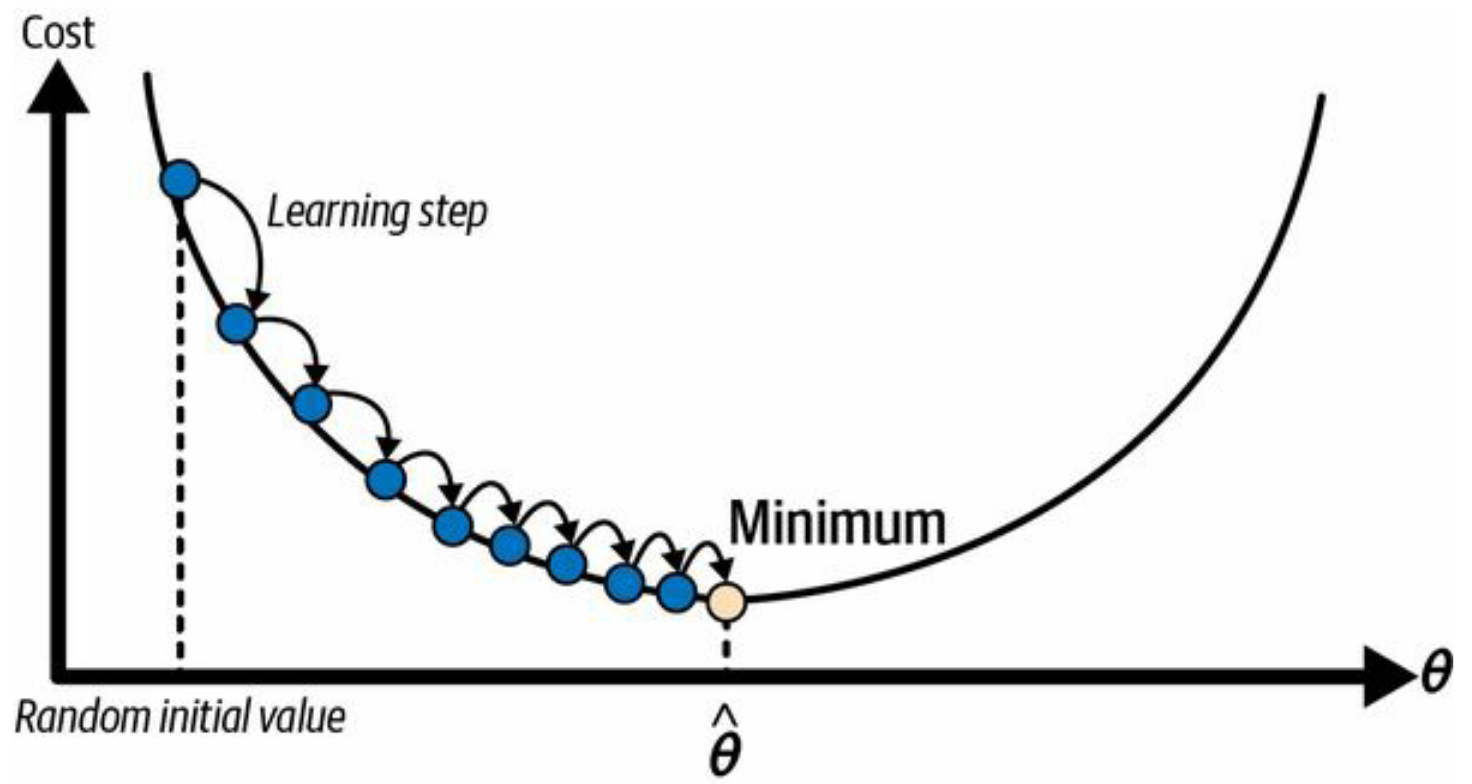
\includegraphics[width=0.5\linewidth, keepaspectratio]{img//chapter4/gradient_descent.png}\label{fig:grad_descent1d}}
  \hfill
  \subfloat[]{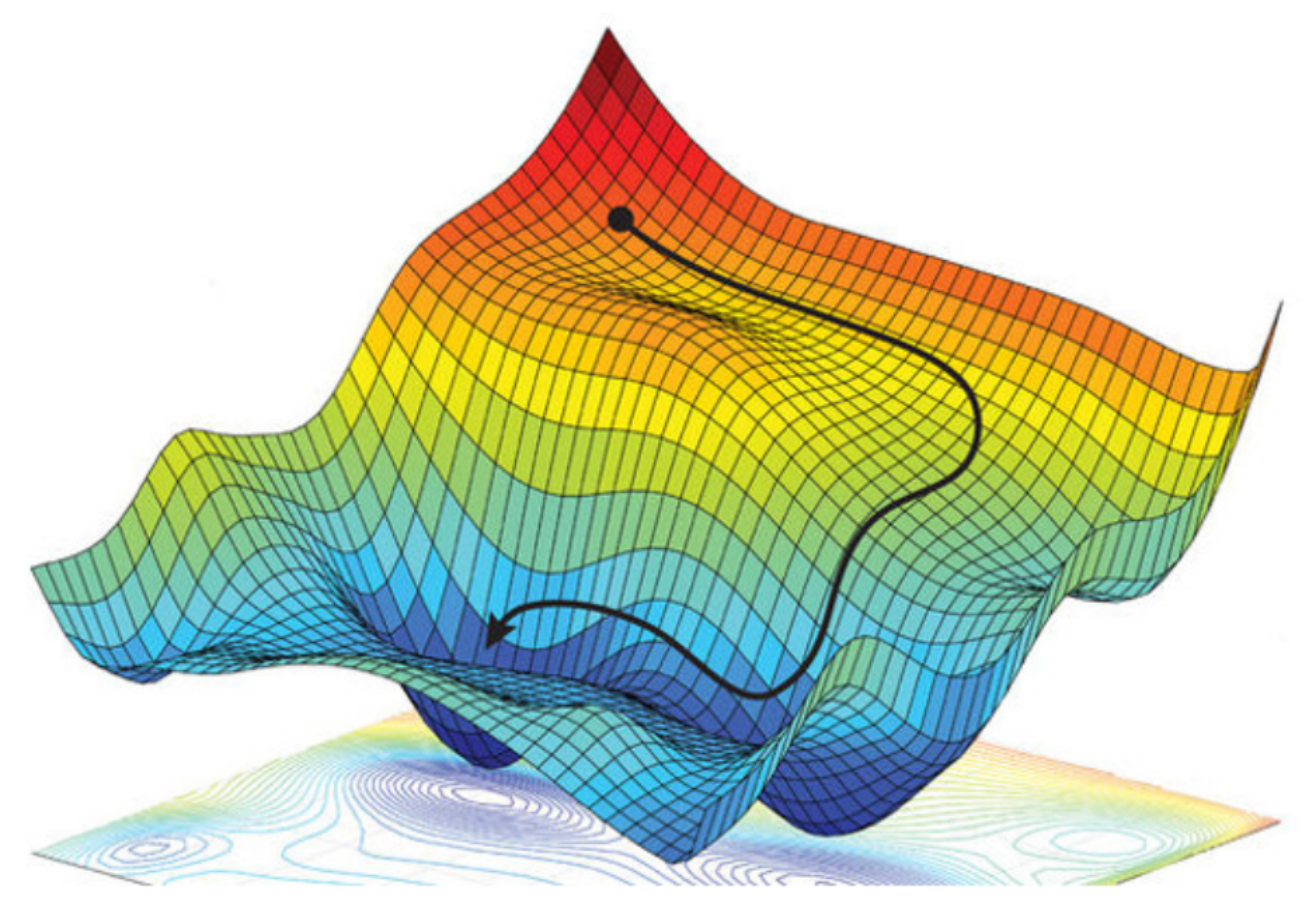
\includegraphics[width=0.5\linewidth, keepaspectratio]{img//chapter4/gradient_descent2d.png}\label{fig:grad_descent2d}}
  \caption[One/two-dimensional gradient descents]{Examples of gradient descents for a \protect\subref{fig:grad_descent1d} one-dimensional loss function and for a \protect\subref{fig:grad_descent2d} two-dimensional one.\\\small{Credits: \cite{geron_hands-machine_2019,amini_spatial_2018}.}}
  \label{fig:grad_descent}
\end{figure}

\begin{figure}
  \centering
  \subfloat[]{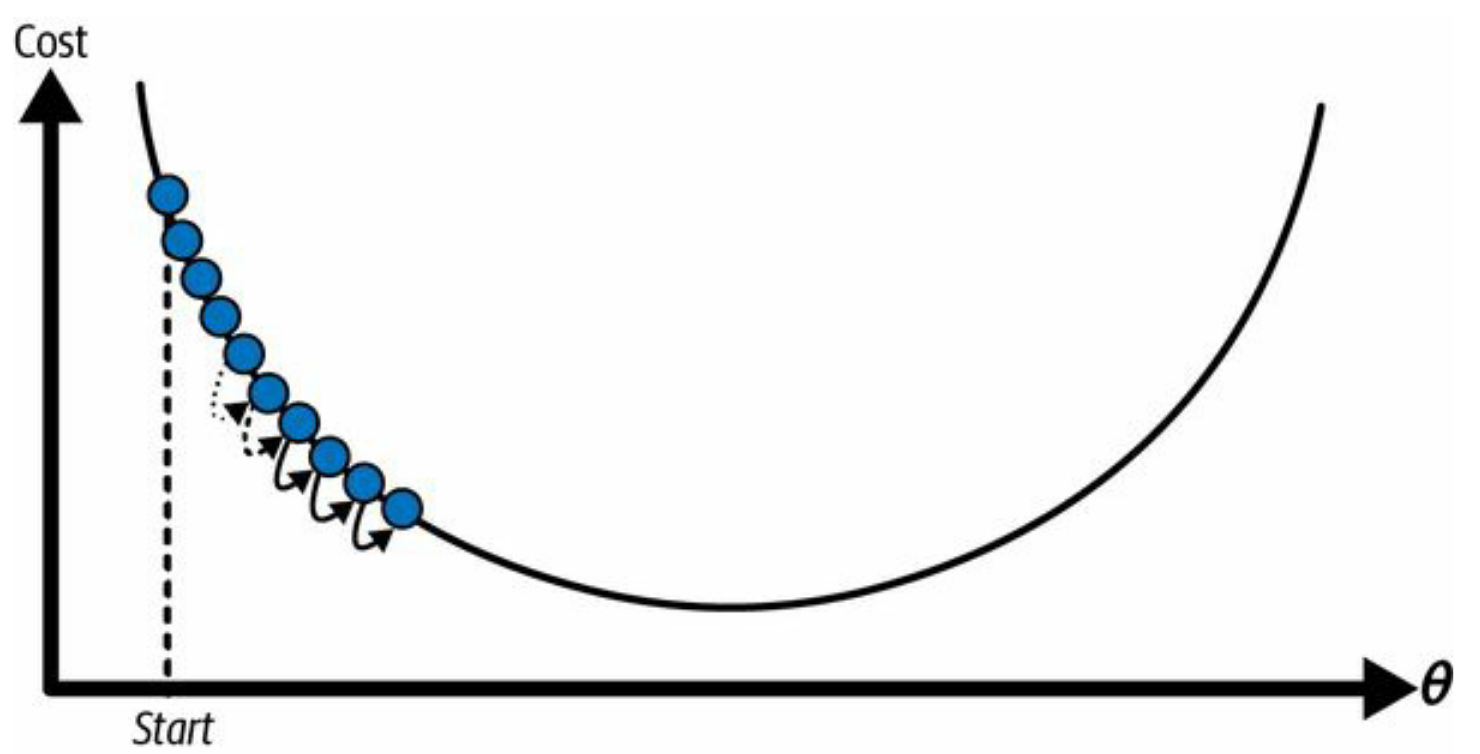
\includegraphics[width=0.5\linewidth, keepaspectratio]{img//chapter4/lr_small.png}\label{fig:lr_small}}
  \hfill
  \subfloat[]{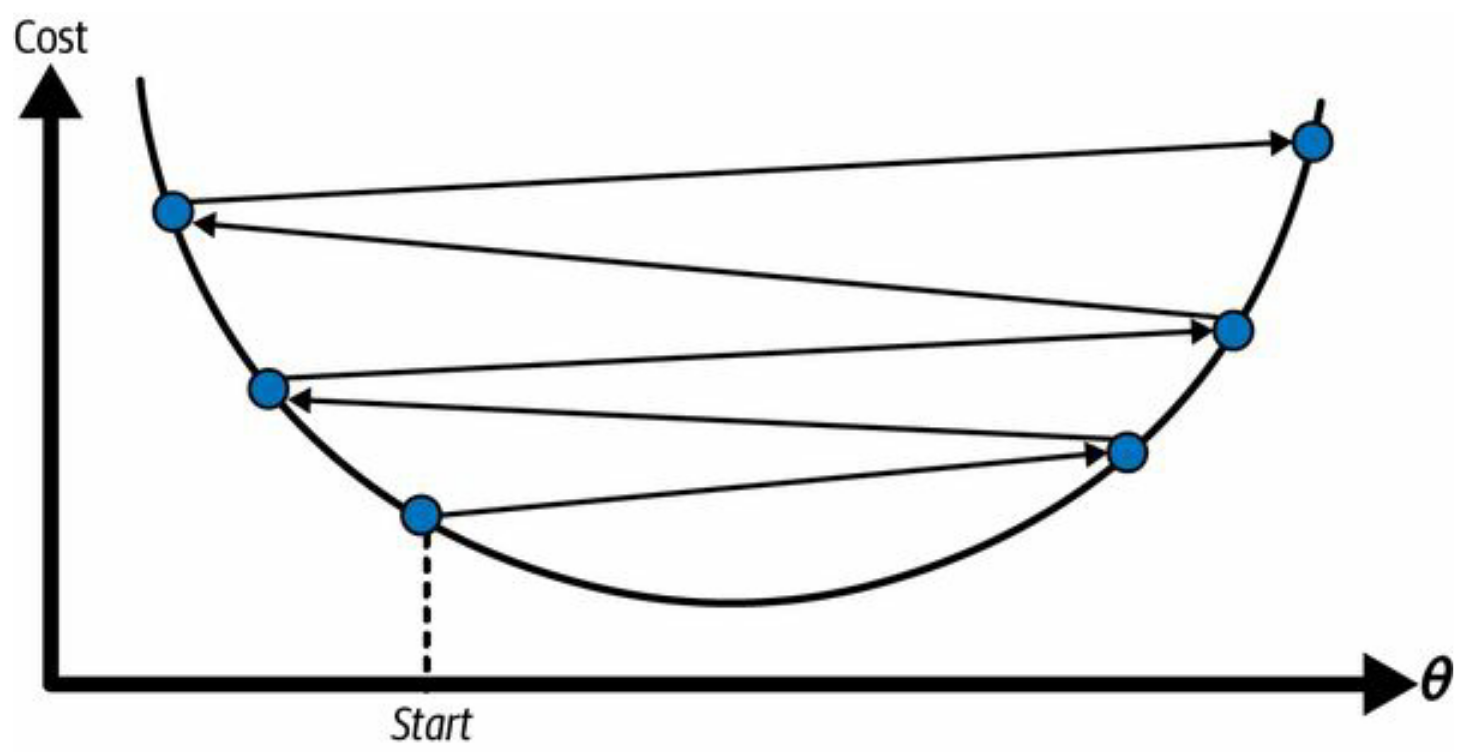
\includegraphics[width=0.5\linewidth, keepaspectratio]{img//chapter4/lr_high.png}\label{fig:lr_high}}
  \caption[Examples of learning rates too small or too high]{Examples of gradient descent for a one-dimensional loss (cost) function with \protect\subref{fig:lr_small} learning rate too small and \protect\subref{fig:lr_high} learning rate too high.\\\small{Credits: \cite{geron_hands-machine_2019}.}}
  \label{fig:lr_small_high}
\end{figure}
\newpage
All gradient-based optimization logic is encapsulated in the \emph{optimizer} object: it determines the direction in which the model parameters should be adjusted and the magnitude of the parameter update (learning rate).

Advanced optimizers, such as Adam \citep{kingma_adam_2017} and AdaDelta \citep{zeiler_adadelta_2012}, go beyond the basic gradient descent by adapting the learning rate during the training process based on the properties of the loss surface (\eg, its curvature). These optimizers can accelerate convergence by dynamically adjusting the step size for each parameter individually, based on the history of gradients. This can be particularly beneficial for navigating complex loss surfaces with varying curvatures.


%%%%%%%%%%%%%%%%%%%%%%%%%%%%%%%%%%%%%%%%%%%%%%%%%%%%%%%
%%%%% SubSubSec: Training loop %%%%%
%%%%%%%%%%%%%%%%%%%%%%%%%%%%%%%%%%%%%%%%%%%%%%%%%%%%%%%
\subsubsection{Training loop}
\label{subsubsec:training_loop}
Having outlined all the essential components within the optimization framework, it is now possible to describe the training process in all its phases, as shown in \cref{fig:backpropagation_algorithm}.
\begin{enumerate}
    \item \textbf{Initialization}: set up the model to be optimized and initialize its parameters to some (random) values.
    \item \textbf{Forward pass}: obtain the model predictions based on the initial parameters and compute the loss to quantify how far the model's outputs are from the actual target/observed values.
    \item \textbf{Backward pass (backpropagation)}: calculate the gradient of the loss function with respect to each parameter in the model. This involves propagating the error backwards from the outputs to the inputs, as described in \cref{subsubsec:reverse_mode}. This process systematically computes the partial derivatives using the chain rule to effectively determine how each parameter should be adjusted to minimize loss.
    \item \textbf{Parameter update (gradient descent)}: for each parameter, update its value by moving it in the direction that minimally decreases the loss
    \be
    \label{eq:4.12}
    \va{\t}_{final} = \va{\t}_{initial} - \eta \va{\nabla}_{\va{\t}_{initial}} f(\va{\t}_{initial}) \,.
    \ee
    \item \textbf{Iteration or convergence}: repeat steps 2 through 4 for a predefined number of iterations (or \emph{epochs}) or until the change in the loss function between iterations falls below a small threshold, indicating convergence.
\end{enumerate}

\begin{figure}
    \centering
    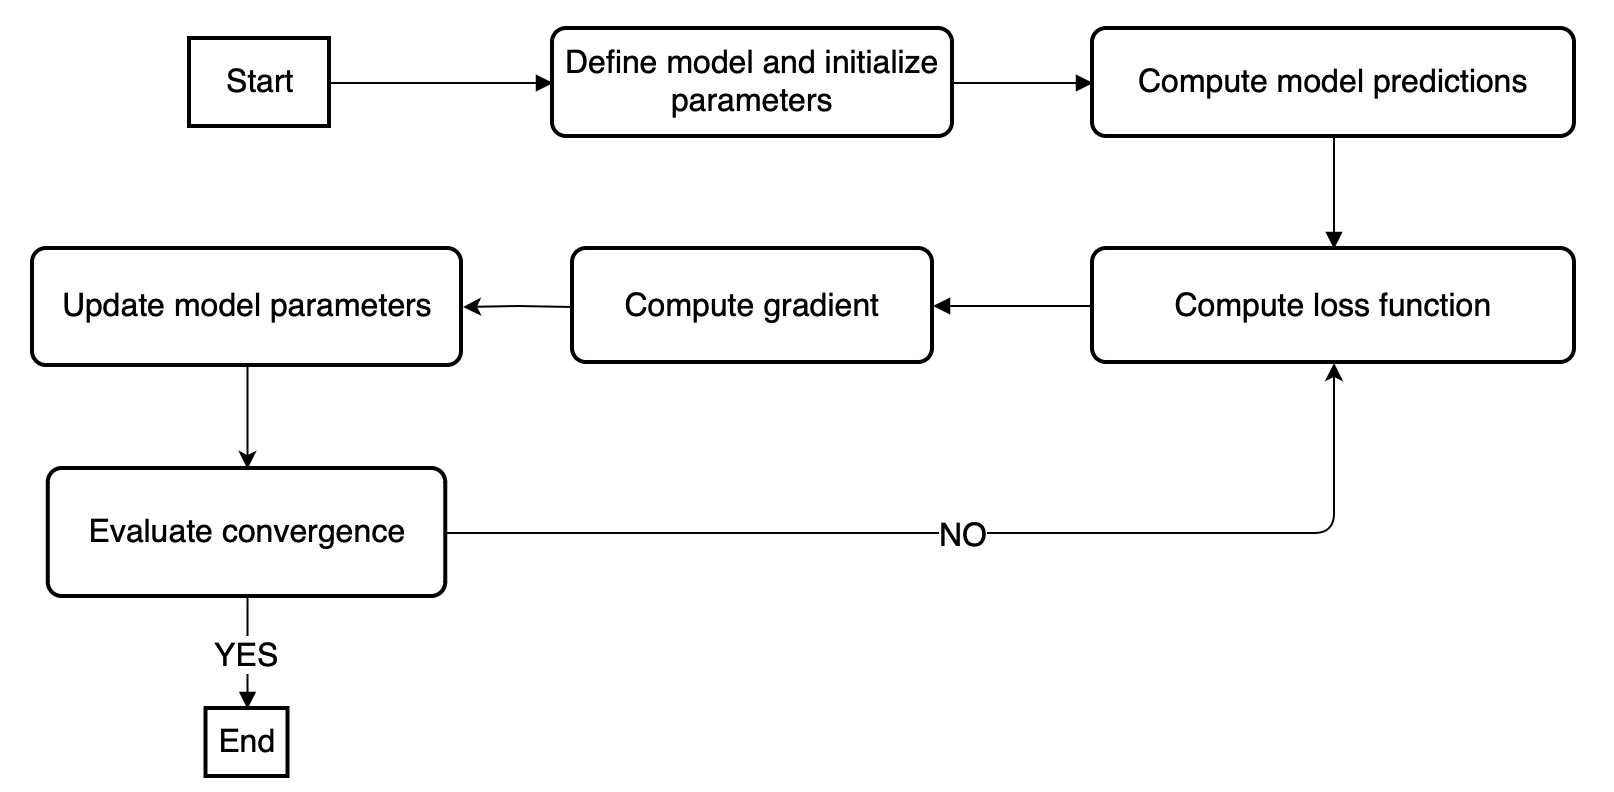
\includegraphics[width=\linewidth, keepaspectratio]{img//chapter4/backpropagation.png}
    \caption[Optimization algorithm diagram]{Optimization algorithm diagram.}
    \label{fig:backpropagation_algorithm}
\end{figure}

The following sections will detail the methods used for the simulation and analysis of the objects presented in \cref{chap:applications}. Beginning with the modeling of light sources and the adopted surface brightness profiles, the discussion will advance to the techniques used for simulating and reconstructing strong gravitational lenses. Finally, methods will be described to assess the accuracy of the model fit to the observed/simulated data.

% *************************************************************
%%%%% SECTION 4.2: LIGHT MODELS %%%%%
%%%%%%%%%%%%%%%%%%%%%%%%%%%%%%%%%%%%%%%%%%%%%%%%%%%%%%%
%%%%% Sec: Light sources modeling  %%%%%
%%%%%%%%%%%%%%%%%%%%%%%%%%%%%%%%%%%%%%%%%%%%%%%%%%%%%%%
\section{Light sources modeling}
\label{sec:light_models}

The prevalent approach to modeling light sources such as galaxies involves using a parametric profile $(R)$, where $R$ represents a measure of distance from the center of the object. These models often presuppose an excessively idealized level of symmetry, yet offer the advantage of being straightforward to define and apply. When building galaxy components, it is generally assumed that the profiles exhibit elliptical symmetry \citep{peng_detailed_2002,peng_detailed_2010}, and therefore $R$ represents the elliptical radius
\be
\label{eq:4.13}
R (\vec{x}^\prime) = \sqrt{{x_1^\prime}^2 + {x_2^\prime / q}^2}
\ee
of a source with an axis ratio $q$. The coordinate system $({x_1^\prime} , {x_2^\prime})$ of the source can be rotated by the \emph{position angle} $\varphi$ with respect to the coordinate system $(x_1 , x_2)$ of the observation. The resulting isophotes\footnote{Curves of constant surface brightness.} of the surface brightness distribution of such an elliptical source are ellipses with semi-major axis $R/q$, semi-minor axis $R$ and orientation $\varphi$ with respect to the $x_1$ axis of observation.


%%%%%%%%%%%%%%%%%%%%%%%%%%%%%%%%%%%%%%%%%%%%%%%%%%%%%%%
%%%%% SubSec: Sérsic profile %%%%%
%%%%%%%%%%%%%%%%%%%%%%%%%%%%%%%%%%%%%%%%%%%%%%%%%%%%%%%
\subsection{Sérsic profile}
\label{subsec:sersic}
The most common model to describe elliptical surface brightness distributions is the \emph{Sérsic law} \citep{sersic_influence_1963,sersic_atlas_1968}, which is given by the exponential
\be
\label{eq:4.14}
I(R) = I_e \exp \bc{- b_n \bs{\bp{\frac{R}{R_{e}}}^{\frac{1}{n}} - 1}} \,,
\ee
where $I_e$ is the surface brightness at the effective radius\footnote{Also called the half-light radius, the radius within which half of the galaxy’s luminosity is contained.} $R_e$ and $n>0$ is called the \emph{Sérsic index}, which characterizes the slope of the profile. The function $b_n$ depends only on the Sérsic index and is defined by
\be
\label{eq:4.15}
\g (2n, b_n) = \frac{1}{2} \G(2n) \,,
\ee
where $\G$, $\g$ are, respectively, the Gamma function and the incomplete Gamma function. It can be shown \citep{ciotti_stellar_1991,ciotti_analytical_1999} that, for a Sérsic index in the range $0.5 \leq n \lesssim 8$, $b_n$ can be approximated by
\be
\label{eq:4.16}
b_n \approx 2n - \frac{1}{3} + \frac{4}{405n} \approx 1.9992n - 0.3271 \,.
\ee
With this, the profile is now fully determined by the seven parameters for position $x_1$, $x_2$, effective radius $R_e$, Sérsic index $n$, intensity at the effective radius $I_e$, axis ratio $q$ and position angle $\varphi$.

The Sérsic profile is a versatile model; by varying $n$ it is possible to obtain many of the classical galaxy profiles as special cases, such as Gaussian profiles ($n = 0.5$), exponential profiles ($n = 1$) and de Vaucouleurs \citep{de_vaucouleurs_recherches_1948} profiles ($n = 4$). 

\begin{figure}
    \centering
    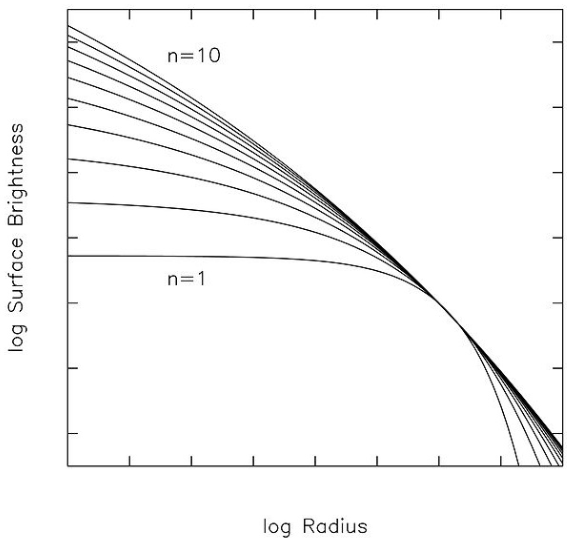
\includegraphics[width=0.65\linewidth, keepaspectratio]{img//chapter4/sersic_n.png}
    \caption[Sérsic profiles for different values of $n$]{Sérsic profiles for different values of $n$. On average, $n \approx 2-10$ for bulges and elliptical galaxies, $n\approx 1$ for disk galaxies and $n \leq 0.5$ for bars and stellar clumps.\\\small{Credits: \cite{burke_assembly_2013}.}}
    \label{fig:sersic_n}
\end{figure}


%%%%%%%%%%%%%%%%%%%%%%%%%%%%%%%%%%%%%%%%%%%%%%%%%%%%%%%
%%%%% SubSec: Core-Sérsic profile %%%%%
%%%%%%%%%%%%%%%%%%%%%%%%%%%%%%%%%%%%%%%%%%%%%%%%%%%%%%%
\subsection{Core-Sérsic profile}
\label{subsec:core_sersic}
An extension of the Sérsic profile has been developed by \cite{graham_new_2003,graham_inner_2004,trujillo_evidence_2004} to better reproduce the observed radial profiles of surface brightness. This model consists of a power law to model the inner radii and a Sérsic function to describe the outer stellar distribution. It is given by
\be
\label{eq:4.17}
I(R) = I^\prime \bs{1 + \bp{\frac{R_b}{R}}^\a}^{\g / \a} \exp{-b_n \bs{\frac{R^\a + R_b^\a}{R_e^\a}}^{1 / (\a n)}} \,,
\ee
where $R_b$ is the break-radius separating the inner power law with logarithmic slope $\g$ from the outer Sérsic profile with slope $n$. The intensity $I_b$ at the break-radius $R_b$ can be evaluated from the expression
\be
\label{eq:4.18}
I^\prime = I_b 2^{- \g / \a} \exp{b_n \bs{\frac{2^{1 / \a} R_b}{R_e}}^{1 / n}} \,.
\ee
The parameter $\a$ controls the sharpness of the transition between the inner (power law) and outer (Sérsic) regimes, with higher values indicating sharper transitions (\cref{fig:core_sersic}).

In this case, the number of parameters becomes larger to include the inner-outer change of regime: the profile is fully determined by ten parameters: for position $x_1$, $x_2$, effective radius $R_e$, Sérsic index $n$, intensity $I_b$ at the break-radius $R_b$, slope of the inner power law $\g$, sharpness of the transition $\a$, axis ratio $q$ and position angle $\varphi$.

\begin{figure}
    \centering
    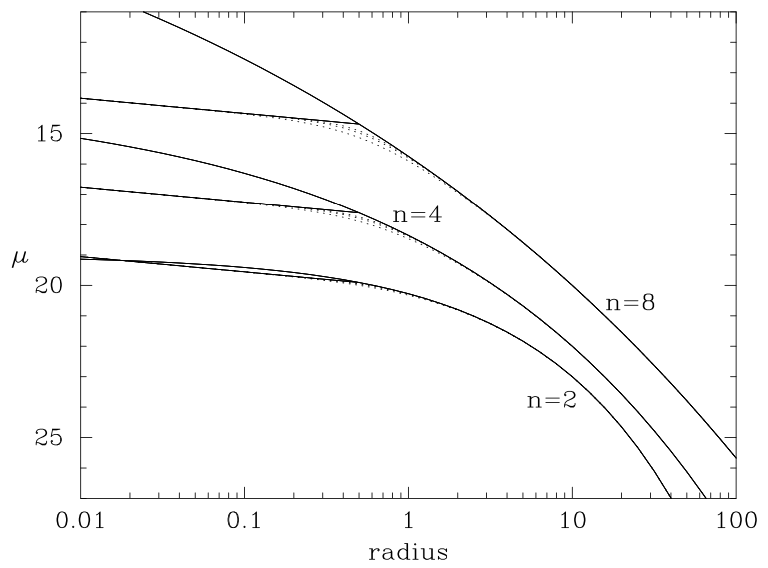
\includegraphics[width=0.7\linewidth, keepaspectratio]{img//chapter4/core_sersic.png}
    \caption[Core-Sérsic profiles for different values of $\a$]{Different core-Sérsic profiles illustrated by the dotted curves for a range of structural parameters. Profiles with values of $\a$ equal to 2, 3, and 4 are shown, the latter giving the sharpest transition. In all models $R_e = \SI{10}{\arcsec}$, $R_b = \SI{0.5}{\arcsec}$, and $\g = 0.2$. For comparison, an inner power law with slope equal to $-0.2$ is shown (diagonal solid lines), as are Sérsic profiles (solid curves) having the same Sérsic shape index $n$.\\\small{Credits: \cite{graham_new_2003}.}}
    \label{fig:core_sersic}
\end{figure}


%%%%%%%%%%%%%%%%%%%%%%%%%%%%%%%%%%%%%%%%%%%%%%%%%%%%%%%
%%%%% SubSec: Sky component  %%%%%
%%%%%%%%%%%%%%%%%%%%%%%%%%%%%%%%%%%%%%%%%%%%%%%%%%%%%%%
\subsection{Sky component}
\label{subsec:sky}
Observations usually include a diffuse distribution of light known as the \emph{sky background}, which must be considered in the reconstruction process. The most basic model for this sky component is a flat surface brightness distribution, characterized by a constant value or a fixed gradient along the $x_1$ and $x_2$ axes of the lens plane. Even if the diffuse background has been removed during a pre-processing step, incorporating a sky component as a free element in the model is advisable. Distinguishing between sky and actual signal is challenging, and any over- or underestimation of the subtracted light can have a considerable impact on the reconstruction outcomes.

%%%%%%%%%%%%%%%%%%%%%%%%%%%%%%%%%%%%%%%%%%%%%%%%%%%%%%%
%%%%% SubSec: Point Spread Function  %%%%%
%%%%%%%%%%%%%%%%%%%%%%%%%%%%%%%%%%%%%%%%%%%%%%%%%%%%%%%
\subsection{Point Spread Function}
\label{subsec:psf}
The Point Spread Function (PSF) is a fundamental concept in optical physics and astronomy that describes how a system blurs or spreads a point light source in an image. The PSF encapsulates the response of an imaging system to a point source or point object, representing the diffraction pattern caused by the optics of the system, including aberrations \citep{bovik_handbook_2005}. Understanding the PSF is crucial for interpreting and processing observational data, as it affects the accuracy with which one can measure the properties of observed objects.

Mathematically, the PSF is often modeled as a convolution kernel that, when applied to an ideal image (the image that would be observed in the absence of any blurring effects), produces the observed image. The process of convolution mathematically
represents spreading the light from point sources over a larger area of the detector, affecting the observed shapes, sizes, and brightness of these objects.

The effect of PSF on an observed image on a plane $(x,y)$ can be described by the convolution of the true image $f(x, y)$ with the Point Spread Function $\mathrm{PSF}(x,y)$, resulting in the observed image $g(x,y)$ \citep{howell_handbook_2006}:
\be
\label{eq:psf}
g(x,y) = (f \ast p)(x,y) = \iint f(x^\prime, y^\prime) \mathrm{PSF}(x - x^\prime, y - y^\prime) \dd{x^\prime} \dd{y^\prime} \,.
\ee


The Point Spread Function (PSF) is usually expressed by means of the Full Width at Half Maximum (FWHM). Their link is rooted in the definition and characterization of the PSF itself. The PSF describes the response of an imaging system to a point source, represented as a distribution or function of intensity across the image plane. The FWHM is a derived characteristic of this distribution, specifically measuring the width of the PSF at half of its maximum intensity.
In the usual case of a Gaussian PSF (\cref{fig:fwhm}):
\be
\label{eq:gauss_psf}
\mathrm{PSF}(x,y) = \mathrm{PSF_0} \exp{- \frac{4 \ln{2}}{\mathrm{FWHM}^2} (x^2 + y^2)} \,,
\ee
where $\mathrm{PSF_0}$ is the peak intensity, the FWHM is directly related to the standard deviation $\s$ of the Gaussian distribution by:
\be
\label{eq:fwhm}
\mathrm{FWHM} = 2 \sqrt{2 \ln{2}} \s \,.
\ee

\begin{figure}
    \centering
    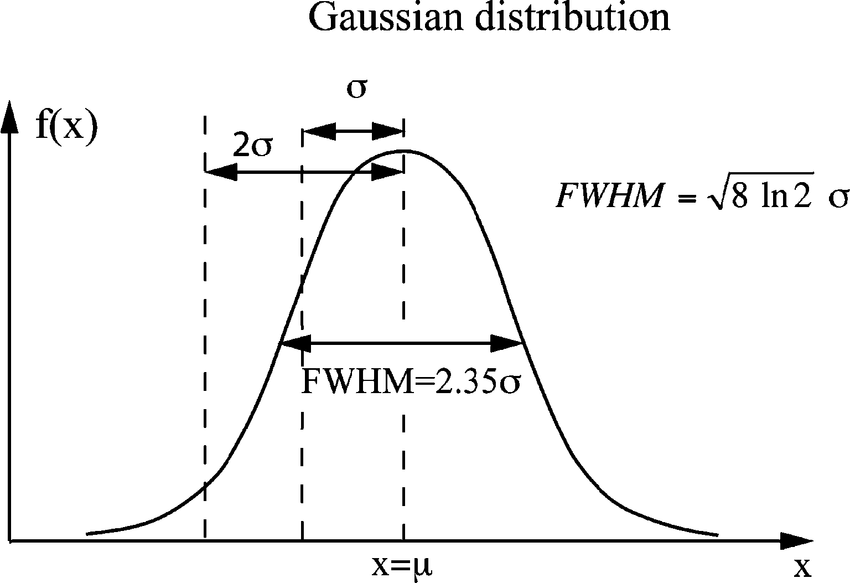
\includegraphics[width=0.6\linewidth]{img//chapter4/fwhm.png}
    \caption[Gaussian PSF and FWHM]{Gaussian or normal PSF and the link with the FWHM.\\\small{Credits: \cite{tavernier_experimental_2010}.}}
    \label{fig:fwhm}
\end{figure}


% *************************************************************
%%%%% SECTION 4.3: LENS INVERSION %%%%%
%%%%%%%%%%%%%%%%%%%%%%%%%%%%%%%%%%%%%%%%%%%%%%%%%%%%%%%
%%%%% Sec: Lens reconstruction  %%%%%
%%%%%%%%%%%%%%%%%%%%%%%%%%%%%%%%%%%%%%%%%%%%%%%%%%%%%%%
\section{Lens reconstruction}
\label{sec:lens_reconstruction}

One of the primary applications of gravitational lensing is reconstructing the lens mass distribution. The modeling of gravitational lenses begins with a collection of observables (\cref{fig:observables}), such as the relative positions and fluxes of images, time delays between images, and other properties of the lens. This modeling can be approached in one of two different but related ways: as a \emph{forward} problem of creating a model of the lens system (lenses and sources) that approximates the observed image the best, or as the \emph{inverse} problem of finding a lens model that deconstructs the observation into a self-consistent and physically viable image of the source. Many successful applications have been published for both the forward \citep{bandara_witnessing_2013,bolton_sloan_2008,newton_sloan_2011,peng_probing_2006} and the inverse method \citep{dye_decomposition_2005,kochanek_lensclean_1992,nightingale_adaptive_2015,suyu_bayesian_2006,vegetti_bayesian_2009,wallington_lensmem_1996,warren_semilinear_2003}.

\begin{figure}
    \centering
    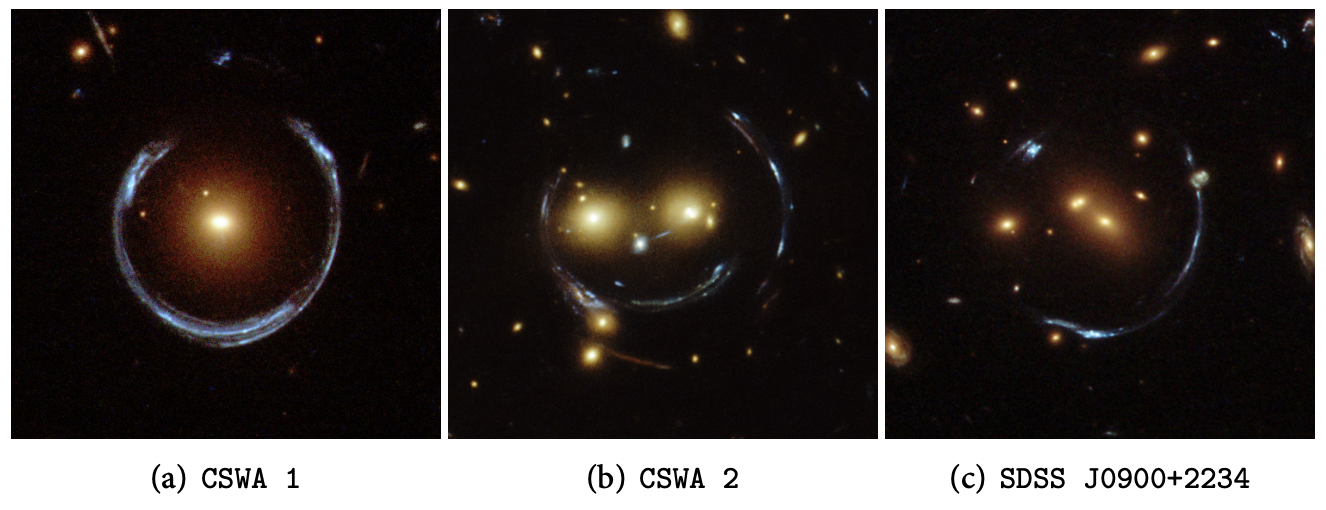
\includegraphics[width=\linewidth, keepaspectratio]{img//chapter4/observables.png}
    \caption[Strong gravitational lensing observations]{Examples of observations of strong gravitational lensing. The large arcs contain information to constrain the gravitational lenses producing these images. \small{Credits: ESA/Hubble $\&$ Nasa}.}
    \label{fig:observables}
\end{figure}

Three types of constraints can be used for this purpose:
\begin{enumerate}
    \item the locations of the multiple images produced by a lensed source help to map out the deflection field of the lens, which corresponds to the first derivatives of the lensing potential \citep{cardone_gravitational_2001}. Obtaining these constraints is relatively straightforward assuming the availability of high-resolution imaging data. This work will mainly focus on this type of constraint.
    \item the magnifications (fluxes) and shapes of the multiple images and gravitational arcs explore the higher-order derivatives (mainly the second) of the lensing potential \citep{gilman_probing_2019}. Therefore, these constraints are particularly sensitive to the smaller-scale mass components of the lens;
    \item the relative time delays between multiple images serve as probes of the lensing potential, as shown in \cref{subsec:time_delay_images}. However, time delays can only be measured in a limited number of lenses (only a few tens) because they require the lensed sources to be intrinsically variable, such as quasars or supernovae \citep{refsdal_possibility_1964}. These types of source are rare. Additionally, measuring time delays is challenging; it demands dedicated telescope time for the continuous observation of these sources over extended periods, along with precise photometry.
\end{enumerate}

The method of translating observed strong lensing constraints into distributions of matter is referred to as lens \emph{inversion} or \emph{reconstruction}.

Such reconstruction is often tackled using two main categories of inversion algorithms \emph{parametric} and \emph{non-parametric} algorithms, based on whether the calculation is ``model-based'' (parametric) or ``model-free'' (non-parametric) at the start of the process \citep{coe_lensperfect_2008}. This work is focused on the first type of approach, applying parametric optimization to retrieve the mass distribution of the lens.

Each approach has its own particular set of strengths and weaknesses, which are summarized here.
\begin{enumerate}

    \item Parametric models employ a clear physical parameterization from the beginning, defining the mass distribution based on a set of specific parameters. Parametric simulation models are generally used to solve the forward problem, taking a source and lensing mass and then predicting the resulting image. Also known as simply-parameterized models, they assume a physical model that fits the data with relatively few defined parameters \citep{jullo_bayesian_2007}. In parametric models, the data is fitted to a physical object (\eg Point-Mass, Singular Isothermal Sphere, Singular Isothermal Ellipsoid, De Vaucouleurs model, etc.) and a model of the lensing mass made using that physical object to predict the effect on the light from the source, often with the assumption that mass follows light. The exploration of these models parameter space aims to identify the optimal combination that accurately replicates the observed positions, shapes, magnitudes, and relative time delays of the multiple images and arcs;

    \item non-parametric methods, which do not start with a predefined physical model but instead use a ``grid-based'' approach, among others, to model the mass distribution. The lens is divided into a mesh, which can be either structured or unstructured, and the lensing observables are projected onto this mesh. Subsequently, this mesh is converted into a pixelized mass distribution using the relationships between the observables and the surface density of the lens. This technique has been extensively applied on a variety of scales, from galaxies to clusters, and has been implemented in numerous ways \citep{birrer_gravitational_2015,blandford_modeling_2000,coles_gravitational_2014,diego_non-parametric_2005,diego_combined_2007,koopmans_gravitational_2005,liesenborgs_genetic_2006,merten_mesh-free_2016,saha_portable_2004,sebesta_testing_2016,suyu_anatomy_2006,suyu_dissecting_2009}.
\end{enumerate}


%%%%%%%%%%%%%%%%%%%%%%%%%%%%%%%%%%%%%%%%%%%%%%%%%%%%%%%
%%%%% SubSec: Parametric reconstruction %%%%%
%%%%%%%%%%%%%%%%%%%%%%%%%%%%%%%%%%%%%%%%%%%%%%%%%%%%%%%
\subsection{Parametric reconstruction}
\label{subsec:parametric_reconstruction}
Strong lensing parametric reconstruction, also known as inversion, involves the use of predefined models to describe both the mass distribution of the lensing object and the light distribution of the background source. The aim is to adjust the parameters of these models to best fit the observed lensing phenomena, such as arcs, rings, and multiple images of a background source. The process is detailed and involves several key steps and algorithms:
\begin{enumerate}
    \item \textbf{model selection} for both the mass distribution and the light distribution;
    \item \textbf{parameter initialization} for the parameters of the mass and light distribution models are made based on observational data or theoretical considerations;
    \item \textbf{ray-tracing simulation} using the initial models: a ray-tracing algorithm computes the deflection angles at each point in the lens plane, which are used to trace the light rays back to the source plane. This step predicts the appearance of the lensed images based on the current model parameters;
    \item \textbf{optimization} via an objective (loss) function that quantifies the difference between the observed and predicted lensed images, as described in \cref{sec:diff_prog}. This function often includes terms for the positions, shapes, and flux ratios of the observed and model-predicted images. Methods such as gradient descent \citep{ruder_overview_2016,canu_introduction_2016}, Markov Chain Monte Carlo (MCMC) \citep{geyer_practical_1992,speagle_conceptual_2019}, or Nested-Sampling \citep{skilling_nested_2004,buchner_nested_2023} are used to adjust model parameters to minimize the objective function. This iterative process refines the model to better fit the observations;
    \item \textbf{model comparison and selection} if multiple models are being tested, and statistical criteria such as the Akaike Information Criterion (AIC) \citep{cavanaugh_akaike_2019} or Bayesian Information Criterion (BIC) \citep{liddle_information_2007,chen_extended_2008} are used to compare their fit to the data, helping to select the best model;
    \item \textbf{uncertainty quantification} for the model parameters, often through bootstrapping or by analyzing the posterior probability distributions in methods like MCMC, providing insights into the confidence levels of the mass and light distribution parameters.
\end{enumerate}

As already stated, parametric reconstruction is highly dependent on the chosen models and their ability to accurately represent the complex mass distributions of astronomical objects. Its strength lies in its relatively straightforward interpretation and the physical significance of the model parameters, but it also faces limitations in flexibility compared to non-parametric methods.

There are several ways to implement parametric lens reconstruction and, as will be shown in \cref{chap:applications}, one of the most common approaches is to use the observed positions of multiple images (\cref{fig:multiple_images_param}).
The optimization can then be performed in mainly two ways: with the so-called \emph{lens} or \emph{image plane optimization} or with the \emph{source plane optimization} technique.

\begin{figure}
    \centering
    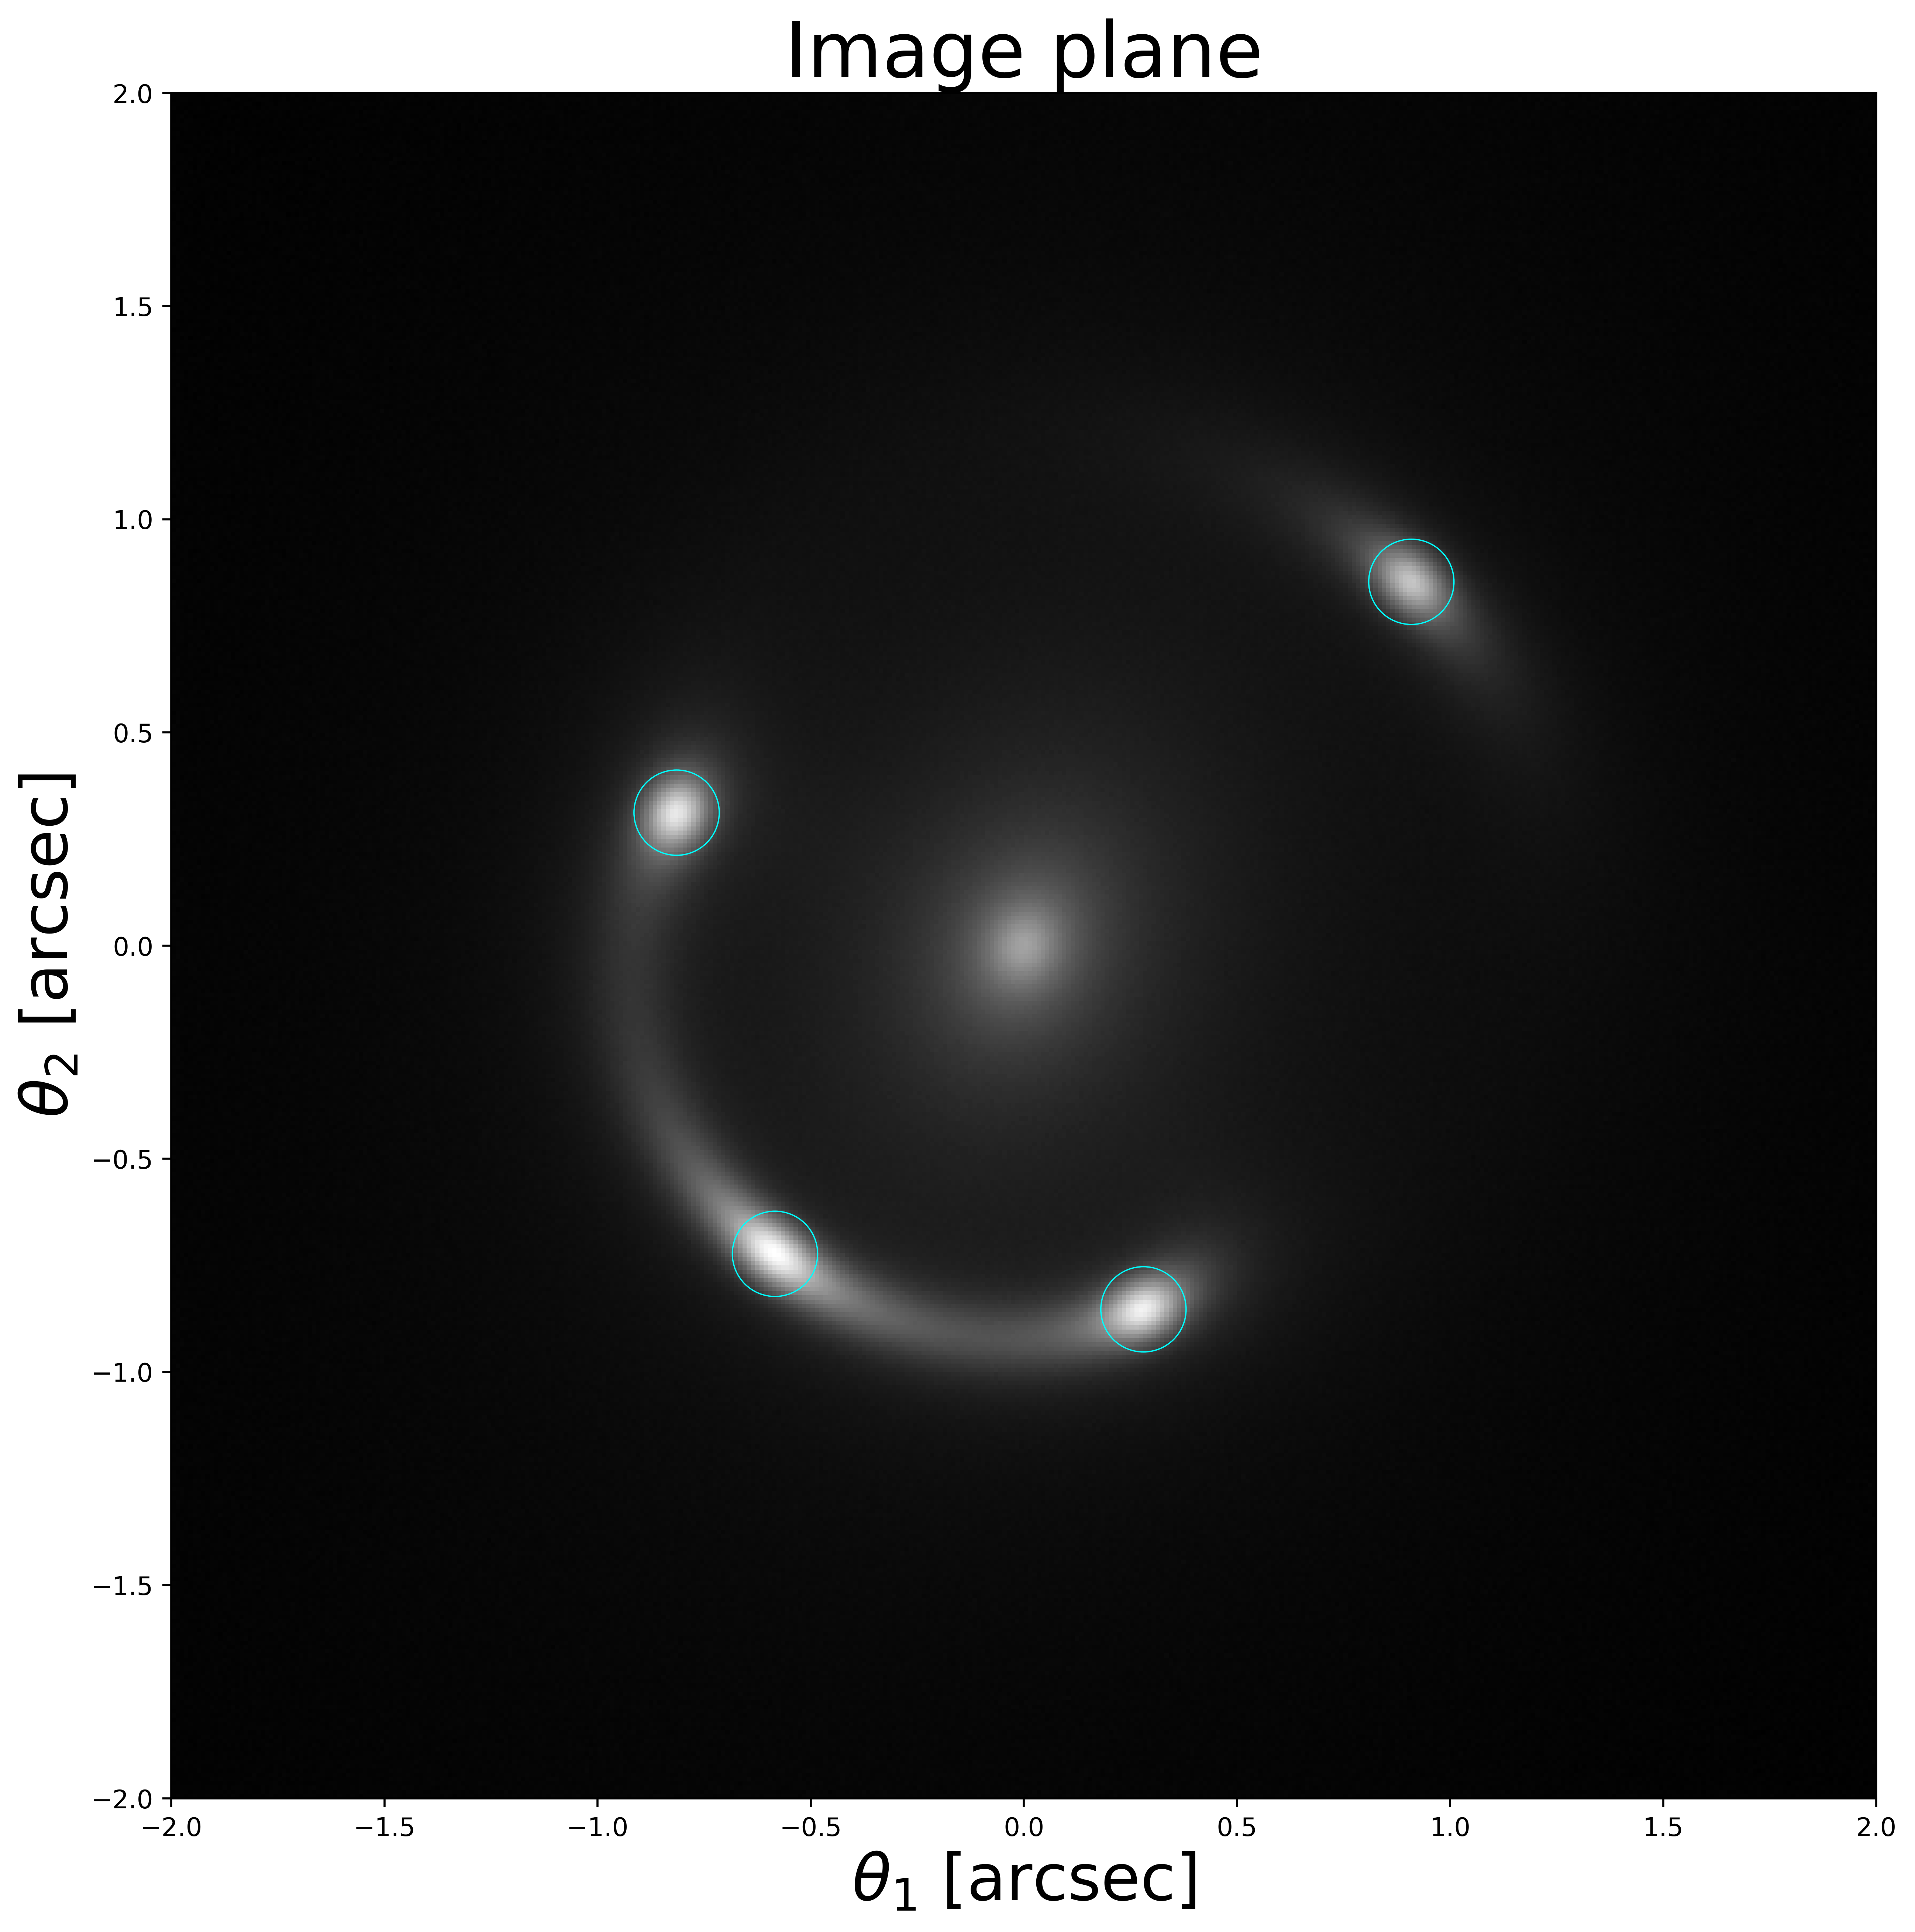
\includegraphics[width=0.6\linewidth, keepaspectratio]{img//chapter4/multiple_images_param.png}
    \caption[Simulated image of a strong lensing event with multiple images]{Simulated image of a strong lensing event with multiple images, indentified by the azure circles. The image is $\SI{4}{\arcsecond} \times \SI{4}{\arcsecond}$, with a pixel scale of $\SI{0.03}{\arcsecond}$.}
    \label{fig:multiple_images_param}
\end{figure}

%%%%%%%%%%%%%%%%%%%%%%%%%%%%%%%%%%%%%%%%%%%%%%%%%%%%%%%
%%%%% SubSubSec: Lens plane and source plane optimization %%%%%
%%%%%%%%%%%%%%%%%%%%%%%%%%%%%%%%%%%%%%%%%%%%%%%%%%%%%%%
\subsubsection{Lens plane and source plane optimization}
\label{subsubsec:lens_plane_source_plane_optimization}
In the context of lens inversion, the positions of multiple images $\va{\t}_i$ are the main observable feature that can be used to constrain the lens parameters. It is assumed that the lens is described by a surface density model (\eg SIS, SIE, etc.) depending on a set of $n$ parameters $\vec{p} = [p_1, \ldots, p_n]$, starting at some initial values (random or constrained by other observables) and that the redshifts of the source and lens are known.

\begin{itemize}
    \item \textbf{Lens plane optimization}

    Given a set of lens parameters, it is possible to calculate the lens deflection angle at the observed positions of the images $\va{\a} (\va{\t}_i | \vec{p})$ and, using the lens equation, map these positions on the source plane:
    \be
    \label{eq:4.19}
    \va{\b}_i (\vec{p}) = \va{\t}_i - \va{\a} ( \va{\t}_i | \vec{p}) \,.
    \ee

    The resulting points $\va{\b}_i (\vec{p})$ will be spread over a certain region in the source plane since the model parameters are not correct. The predicted source position can be estimated by taking the mean position of these points:
    \be
    \label{eq:4.20}
    \va{\b} (\vec{p}) = \frac{1}{N_{ima}} \sum\limits_{i=1}^{N_{ima}} \va{\b}_i (\vec{p}) \,,
    \ee
    where $N_{ima}$ is the observed number of multiple images.

    Subsequently, by solving the lens equation, the predicted source position can be mapped back to the lens plane, obtaining a set of predicted image positions
    \be
    \label{eq:4.21}
    \va{\b} (\vec{p}) \rightarrow \{\va{\t}_i (\vec{p}) ; i = 1, \ldots, N_{ima, \vec{p}}\} \,,
    \ee
    where the number of predicted images, $N_{ima, \vec{p}}$, can clearly be different from $N_{ima}$.

    At this point a cost function can be defined to compare the predicted and observed positions of the images
    \be
    \label{eq:4.22}
    \chi^2 (\vec{p}) = \sum\limits_{i=1}^{N_{ima}} \frac{[\va{\t}_i - \va{\t}_i (\vec{p})]^2}{\s_i^2} \,,
    \ee
    where $\va{\t}_i (\vec{p})$ is the position of the predicted image closest to the image at $\va{\t}_i$ and $\s_i$ is the error on the position of the $i$-th image.

    To identify the optimal lens model, one can adjust the parameters $\vec{p}$ to minimize the loss function, or equivalently, to maximize the likelihood of the observed image positions given the parameters $\vec{p}$
    \be
    \label{eq:4.23}
    \mathscr{L} (\vec{p}) = \frac{1}{\prod\limits_{i=1}^{N_{ima}} \s_i \sqrt{2 \pi}} \exp \left[ - \frac{\chi^2 (\vec{p})}{2} \right] \,.
    \ee

    When dealing with multiple families of multiple images, the same approach can be utilized. However, the likelihood function must be adjusted to become the product of the likelihoods corresponding to each image family
    \be
    \label{eq:4.24}
    \mathscr{L} (\vec{p}) = \prod\limits_{j=1}^{N_{fam}} \frac{1}{\prod\limits_{i=1}^{N_{ima}} \s_{ji} \sqrt{2 \pi}} \exp \left[ - \frac{\chi_j^2 (\vec{p})}{2} \right] \,,
    \ee
    with $\chi_j^2$ as defined in \cref{eq:4.22}, but referring to the $j$-th family of multiple images and $\s_{ji}$ is the error on the position of the $i$-th image of the $j$-th family.

    Maximizing the aforementioned likelihood is equivalent to minimizing the total chi-squared value $\chi_{tot}^2$, which is defined by
    \be
    \label{eq:4.25}
    \chi_{tot}^2 (\vec{p}) = \sum\limits_{j=1}^{N_{fam}} \chi_j^2 (\vec{p}) \,.
    \ee
    \clearpage
    \item \textbf{Source plane optimization}

    An alternative to optimizing in the lens plane is to perform optimization in the source plane. In an ideal scenario, if the model parameters precisely match the lens parameters, multiple images would map to a single position on the source plane. Consequently, a cost function can this time be defined on the source plane to facilitate this optimization process
    \be
    \label{eq:4.26}
    \chi_s^2 (\vec{p}) = \sum\limits_{i=1}^{N_{ima}} \frac{[\va{\b}_i (\vec{p}) - \va{\b} (\vec{p})]^2}{ \s_i^2} \mu_i (\vec{p})^2 \,,
    \ee
    where $\mu_i (\vec{p})$ is the model estimated magnification at the $i$-th image position.
\end{itemize}


The primary benefit of source plane optimization is the elimination of the most complex step in the previously described lens plane optimization procedure. This step, which involves solving the lens equation, can be computationally intensive and is typically addressed by numerical methods. When leveraging multiple families of images as constraints, optimization on the lens plane becomes considerably more time consuming compared to source plane optimization. Furthermore, this approach does not require a one-to-one match between the observed and predicted images by the model when calculating the chi-squared $\chi^2$. However, a potential downside is that the error for each predicted source position $\b_i (\vec{p})$ must be estimated using the model-predicted magnification $\mu_i (\vec{p}) = \mu (\va{\t}_i | \vec{p})$ at the image positions. Additionally, optimization on the source plane may produce biased solutions, often favoring models with flatter density profiles and higher ellipticity \citep{kneib_cluster_2011}.
